\documentclass{beamer}
\usepackage[utf8]{inputenc}
\usepackage{graphicx}
\usetheme{Madrid}

\usepackage[n, advantage, operators, sets, adversary, landau, probability, notions, logic, ff, mm, primitives, events, complexity, asymptotics, keys] {cryptocode}


\title{Security of Deterministic Encryption}
\author[Zichen]{Zichen Gui\\{\small Supervised by: Dr. Bogdan Warinschi}}


\begin{document}

\frame{\titlepage}

\begin{frame}{Outline of the presentation}
\begin{itemize}
\item Introduce to encryption schemes with additional properties
\item Describe deterministic encryption scheme
\item Demonstrate usefulness of deterministic encryption
\item Analyse the security of deterministic encryption
\item Show that deterministic encryption is not secure in database applications
\item Discuss the approaches of the research
\end{itemize}
\end{frame}	


\begin{frame}{Introduction}
\begin{itemize}
\item Security of traditional encryption schemes are based on indistinguishability (IND) of ciphertexts or semantic security
\item In particular, they need to be probabilistic
\item Not efficient for processing encrypted data
\end{itemize}
\end{frame}


\begin{frame}{Introduction}
\begin{itemize}
\item Schemes allowing for better processing of encrypted data often process some additional properties
\item Usual security notion of IND cannot be satisfied
\item Need to understand the maximal level of security those schemes can offer
\end{itemize}
\end{frame}


\begin{frame}{Construction of deterministic encryption (1)}
\begin{itemize}
\item Based on a (secure) hash function $H$ and a probabilistic encryption scheme $(\mathcal{K}, \mathcal{E}, \mathcal{D})$

\begin{figure}[H]
	\begin{pchstack}[center]
		\procedure{Key generation}{%
			\pcln (\pk, \sk) \sample \mathcal{K}(1^n)
		}
		
		\pchspace
		
		\procedure{Encryption(\pk, $x$)}{%
			\pcln \omega \gets H(\pk \concat x)       \\
			\pcln y \gets \mathcal{E}(\pk, x; \omega) \\
			\pcln \pcreturn y
		}
		
		\pchspace
		
		\procedure{Decryption(\pk, \sk, $y$)}{%
			\pcln x \gets \mathcal{D}(\sk, y)  \\
			\pcln \omega \gets H(\pk \concat x)  \\
			\pcln \pcif \mathcal{E}(\pk, x; \omega) = y \\
			\pcln\text{\t} \pcreturn x  \\
			\pcln \pcreturn \perp
		}
	\end{pchstack}
	
	\caption{Deterministic encryption based on hashing}
\end{figure}

\end{itemize}
\end{frame}


\begin{frame}{Construction of deterministic encryption (2)}
\begin{itemize}
\item Use trapdoor permutation in place of hash function
\item Trapdoor permutation is a family of functions that is easy to compute but hard to invert
\item If given some additional information, known as the 'trapdoor', the inversion can be computed efficiently
\end{itemize}
\end{frame}


\begin{frame}{Construction of deterministic encryption (2)}
\begin{figure}
	\begin{pchstack}[center]
		\procedure{Key generation}{%
			\pcln (\phi, \tau) \sample \mathcal{G}(1^n)  			    \\
			\pcln s \sample \{0, 1\}^n   								\\
			\pcln (\bar{\pk}, \bar{\sk}) \sample \mathcal{K}(1^n)       \\
			\pcln \pk \gets (\phi, \bar{\pk}, s)                        \\
			\pcln \sk \gets (\tau, \bar{\sk})             				\\
			\pcln \pcreturn (\pk, \sk)
		}
		
		\pchspace
		
		\procedure{Encryption(\pk, $x$)}{%
			\pcln (\phi, \bar{\pk}, p) \gets \pk        \\
			\pcln y \gets F(\phi, x)                    \\
			\pcln \omega \gets GetCoins(F, \phi, x, s)  \\
			\pcln c \gets \mathcal{E}(\pk, y; \omega)   \\
			\pcln \pcreturn c
		}
	\end{pchstack}
	
	\caption{Deterministic encryption based on trapdoor permutations}
	

\end{figure}
\end{frame}


\begin{frame}{Construction of deterministic encryption (2)}
\begin{figure}
	\begin{pchstack}[center]
		\procedure{Decryption(\pk, \sk, $y$)}{%
		\pcln (\tau, \bar{\sk}) \gets \sk        \\
		\pcln y \gets \mathcal{D}(\bar{\sk}, c)  \\
		\pcln x \gets \bar{F}(\tau, y)           \\
		\pcln \pcreturn x
	}
	\end{pchstack}

	\caption{Deterministic encryption based on trapdoor permutations}
\end{figure}
\end{frame}


\begin{frame}{Usefulness of Deterministic Encryption}
\begin{itemize}
\item Overcomes poor source of randomness used in probabilistic encryption schemes
\item Allows for efficient searching in databases: \\
- log-time with binary trees such as red-black tree or 2,3,4-tree  \\
- log-log-time with Van Emde Boas tree
\end{itemize}	
\end{frame}


\begin{frame}{Security of Deterministic Encryption}{Original definition}
\begin{itemize}
\item An IND adversary is a triple $I = (I_c, I_m, I_g)$ of PPT algorithms
\item $I_c$: generates a state that will be used by $I_m$
\item $I_m$: generates a pair of messages given the state
\item $I_g$: guess the challenge bit $b$
\end{itemize}
\end{frame}


\begin{frame}{Security of Deterministic Encryption}{Original definition}
\begin{figure}[H]
	\begin{pchstack}[center]
		\procedure{Experiment $\text{EXP}_\text{I}^\text{IND}(n)$}{%
			\pcln st \gets I_c(1^n)        \\
			\pcln (m_0, m_1) \gets I_m(st) \\
			\pcln b \sample \{0, 1\}       \\
			\pcln c \gets \text{Encryption}(pk, m_b) \\
			\pcln b^{'} \gets I_g(\pk, c, st)
		}
	\end{pchstack}
	
	\caption{IND game for deterministic encryption}
\end{figure}
\end{frame}


\begin{frame}{Security of Deterministic Encryption}{Original definition}
Differences to the standard IND security:
\begin{itemize}
	\item
	The algorithms $I_c$ and $I_m$ accessed by the adversary have no access to the public key.
	\item
	The final algorithm $I_g$ only has access to the state generated by $I_c$, instead of the plaintexts $(m_0, m_1)$.
	\item
	The message space has high min-entropy.
\end{itemize}
\end{frame}


\begin{frame}{Security of Deterministic Encryption}{Alternative definition}
\begin{figure}[H]
	\begin{center}
		\begin{bbrenv}{B}
			\begin{bbrbox}[name=Adversary, minheight=3.5cm, minwidth=2.5cm]
			\end{bbrbox}
			
			\bbrmsgfrom{top = {$\{(m_0^{i}, m_1^{i})\}$}, length=2cm}
			\bbrmsgspace{1cm}
			\bbrmsgto{top = {$\{c_b^{i}\}$}, length=2cm}
			\bbrmsgspace{1cm}
			\bbrmsgfrom{top = {$b'$}, length=2cm}
			
			\begin{bbroracle}{OraA}
				\begin{bbrbox}[name={Encryption}, minheight=1cm]
				\end{bbrbox}
			\end{bbroracle}
			\bbroracleqryto{top= {$m$}}
			\bbroracleqryfrom{top = {$Enc(m)$}}
			
		\end{bbrenv}
	\end{center}
	
	\caption{Cryptographic game of IND-DCPA}
\end{figure}
\end{frame}


\begin{frame}{Attack on deterministic encryption in databases}
\begin{itemize}
\item Deterministic encryption leaks frequency
\item Frequency of ciphertexts can be compared to auxiliary data or prior knowledge to match the ciphertexts to plaintexts
\begin{figure}
	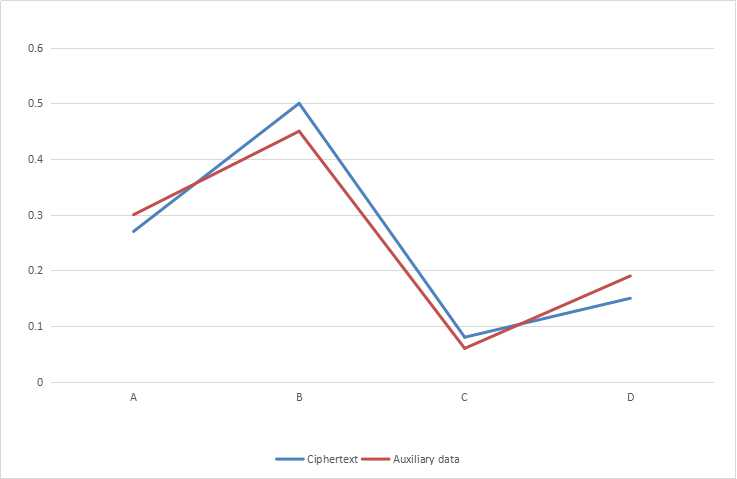
\includegraphics[width=0.5\textwidth]{./attack.jpg}
	\caption{Attack by comparing frequency of some auxiliary data and ciphertexts}
\end{figure}
\end{itemize}
\end{frame}


\begin{frame}{Summary}
In the presentation, we have discussed:
\begin{itemize}
\item Construction of deterministic encryption (DE)
\item Usefulness of DE in database applications
\item DE is not secure in database applications
\end{itemize}
\end{frame}


\begin{frame}{Discussion}
Scientific questions to be addressed in the project:
\begin{itemize}
\item How should security notion be defined for DE in application to databases?
\item Is there an encryption scheme that is secure under that security definition?
\end{itemize}
\end{frame}






\end{document}